\section{Model Exercise 2-1b (02): Fluid driven percolation in clay}
\label{sec:mex2-1b}
%------------------------------------------------------------------------------
\Authors{Amir Sattari, Keita Yoshioka et al.}
%------------------------------------------------------------------------------
In this model exercise, the fracking path and fracking pressure for a sandy Opalinus claystone sample under two different initial stress configurations are investigated. In addition to the stress configurations and due to the high anisotropy of the claystone samples, it is expected that due to the weak bond between the embedded layers, the fracking path and flow will be governed by orientation of the embedded layers.  

%------------------------------------------------------------------------------
\subsection{Experimental set-up}
%------------------------------------------------------------------------------

The cubic Opalinus claystone samples are prepared in the side dimension of 43 $mm$ and with the drilled cavity length and diameter of 20 and 8 $mm$ (Figure \ref{fig:Amir_Percolation_Adapter}). The applied mechanical stress configurations are as shown in Fig. \ref{fig:Amir_Percolation_Stress_1} and \ref{fig:Amir_Percolation_Stress_2}. The samples embedded layering orientations are shown in Fig. \ref{fig:Amir_Percolation_Orientation1} and \ref{fig:Amir_Percolation_Orientation2}, where in the first case the applied oil pressure is perpendicular to the layering orientations and in the second case it is parallel to the layering orientations.

\begin{figure}[!ht]
\begin{subfigure}[c]{0.48\textwidth}
\centering
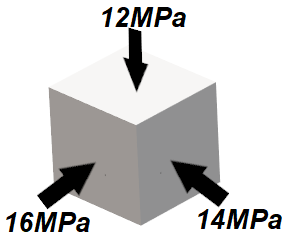
\includegraphics[width=5cm,height=4cm]{figures/Amir_Percolation_Stress_1.png}
\subcaption{}
\label{fig:Amir_Percolation_Stress_1}
\end{subfigure}
\hfill
\begin{subfigure}[c]{0.48\textwidth}
\centering
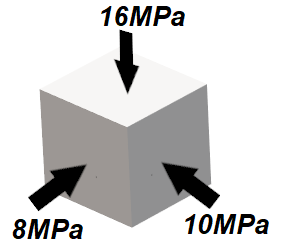
\includegraphics[width=5cm,height=4cm]{figures/Amir_Percolation_Stress_2.png}
\subcaption{}
\label{fig:Amir_Percolation_Stress_2}
\end{subfigure}
\caption{The applied (a) $1^{st}$, and (b) the $2^{nd}$ stress configurations}
\end{figure}

\begin{figure}[!ht]
\begin{subfigure}[c]{0.48\textwidth}
\centering
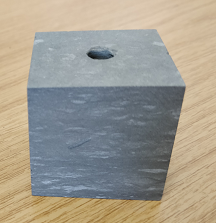
\includegraphics[width=4cm,height=4cm]{figures/Amir_Percolation_Orientation1.png}
\subcaption{}
\label{fig:Amir_Percolation_Orientation1}
\end{subfigure}
\hfill
\begin{subfigure}[c]{0.48\textwidth}
\centering
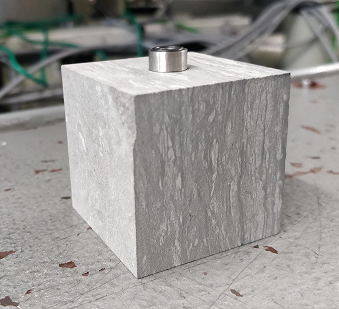
\includegraphics[width=4cm,height=4cm]{figures/Amir_Percolation_Orientation2.png}
\subcaption{}
\label{fig:Amir_Percolation_Orientation2}
\end{subfigure}
\caption{The orientation of the embedded layers (a) perpendicular, and (b) parallel to the direction of the borehole pressure configuration}
\end{figure}


The syringe pump is used to pump the pressurized hydraulic oil (up to 517 $Bar$) into the sample and with gradually increasing the pressure the fracking process is carried out. In the first setup, the hydraulic fracking is initiated at 23 $MPa$ and the clear flow paths through the embedded layering surfaces is observed \ref{fig:Amir_Percolation_Frack_a}. Similarly, for the second test setup, the hydraulic fracking is initiated at 10 $MPa$ through the embedded layering surfaces as shown in Fig. \ref{fig:Amir_Percolation_Frack_b}. Fig. \ref{fig:Amir_Percolation_Flow_a} and \ref{fig:Amir_Percolation_Flow_b} illustrates the borehole pressure evolution with flow volume change obtained from the experimental data. The initial volume of the pump is around 265 $mL$,


\begin{figure}[!ht]
\begin{subfigure}[c]{0.48\textwidth}
\centering
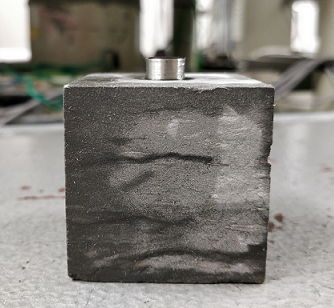
\includegraphics[width=5cm,height=5cm]{figures/Amir_Percolation_Frack_a.png}
\subcaption{}
\label{fig:Amir_Percolation_Frack_a}
\end{subfigure}
\hfill
\begin{subfigure}[c]{0.48\textwidth}
\centering
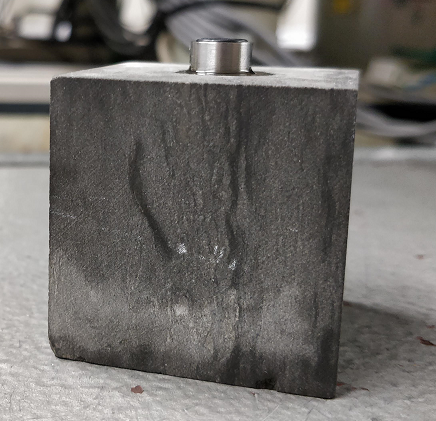
\includegraphics[width=5cm,height=5cm]{figures/Amir_Percolation_Frack_b.png}
\subcaption{}
\label{fig:Amir_Percolation_Frack_b}
\end{subfigure}
\caption{The fracking paths through the Opalinus claystone (a) $1^{st}$ stress configuration, and (b) $2^{nd}$ stress configuration}
\end{figure}

\begin{figure}[!ht]
\begin{subfigure}[c]{0.48\textwidth}
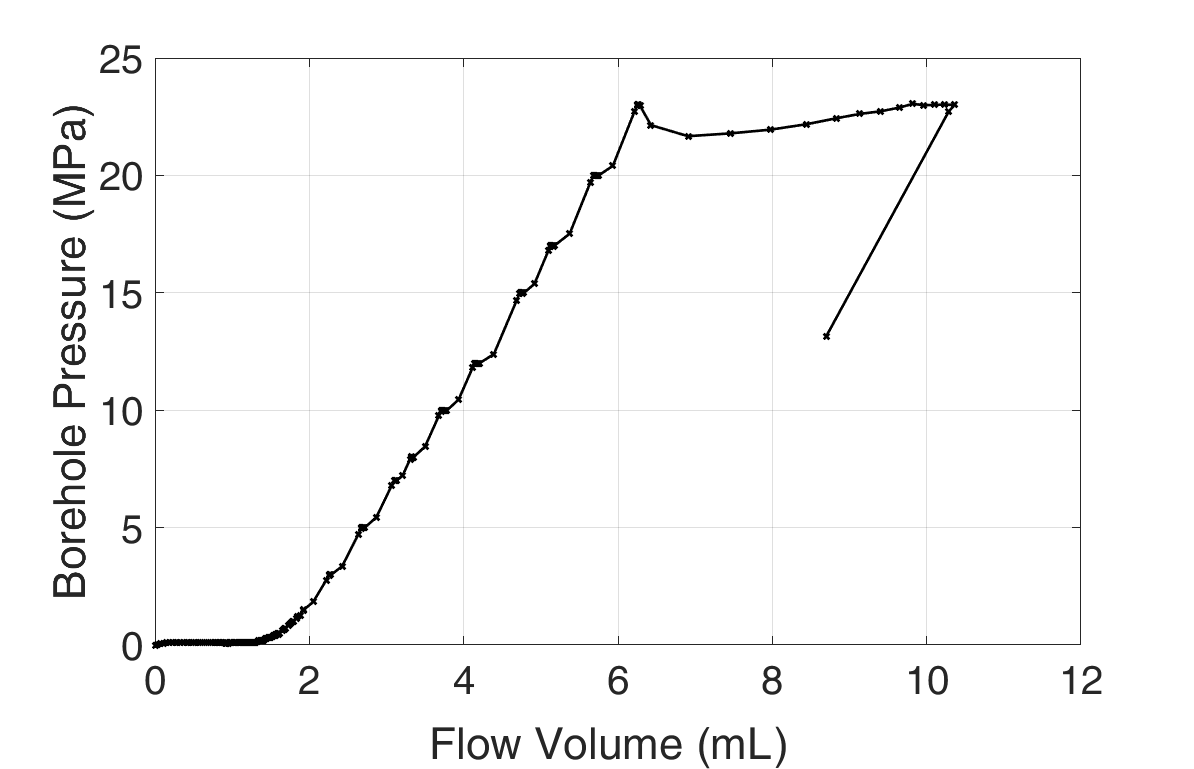
\includegraphics[width=1\textwidth]{figures/Amir_Percolation_Flow_a.png}
\subcaption{}
\label{fig:Amir_Percolation_Flow_a}
\end{subfigure}
\hfill
\begin{subfigure}[c]{0.48\textwidth}
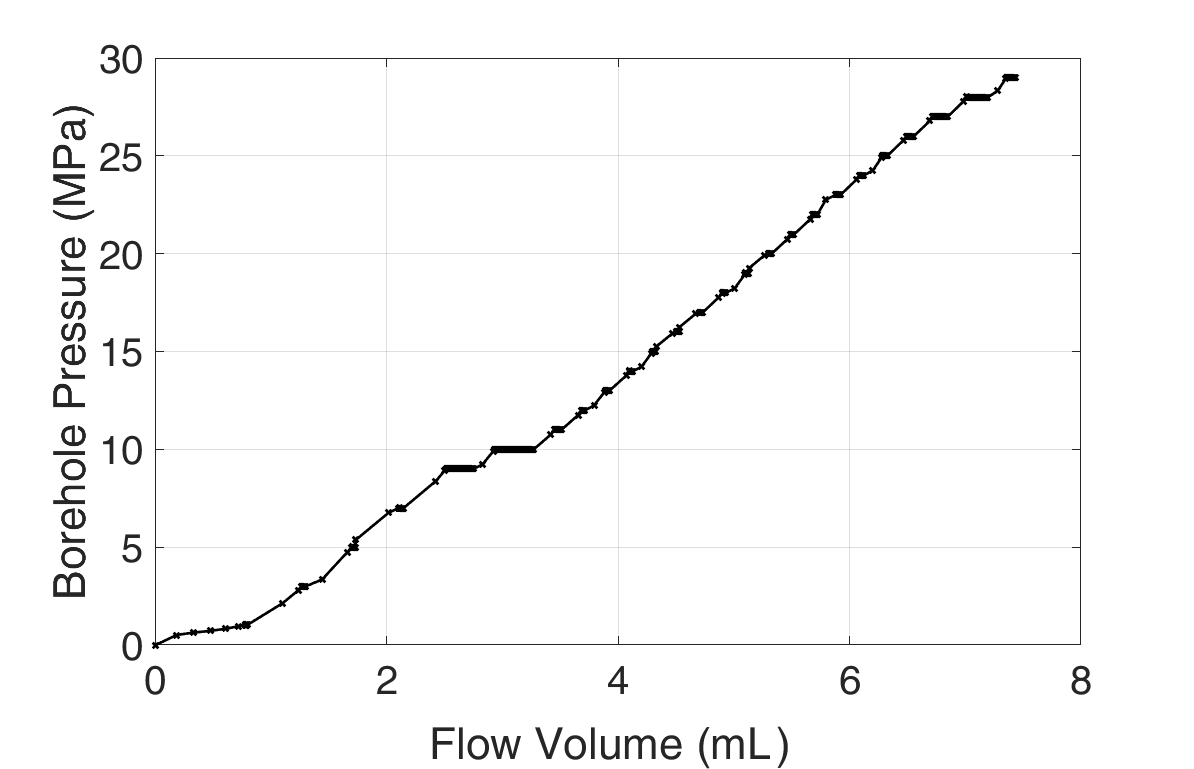
\includegraphics[width=1\textwidth]{figures/Amir_Percolation_Flow_b.png}
\subcaption{}
\label{fig:Amir_Percolation_Flow_b}
\end{subfigure}
\caption{The borehole pressure vs. flow volume for a Opalinus claystone (a) $1^{st}$ stress configuration, and (b) $2^{nd}$ stress configuration}
\end{figure}

%------------------------------------------------------------------------------
\subsection{Model approaches}
%------------------------------------------------------------------------------
\subsubsection*{Lattice-Element-Model (LEM)}

With the implemented lattice model, the effect of the Opalinus claystone anisotropy on the fracking paths and fracking pressure is investigated. The similar approach as described in section \ref {sec:mex01} is taken to define the layering orientations in the medium. It is assumed that the interface elements bonding two different layers have 5 times weaker strength than the same layers bond (found in \ref{sec:Brazilian_Disk_Exp}). The generated 3D setup using the LEM is shown in Fig. \ref{fig:Amir_Percolation_Setup_a} and \ref{fig:Amir_Percolation_Setup_b}. The total number of mechanical and conduct lattice elements are approximately 28000 and 200000, respectively.
The percolation tests under the two stress configurations and with different embedded layering orientations are simulated. Fig. \ref{fig:Amir_ME2_B_Fracture_a} and \ref{fig:Amir_ME2_B_Fracture_b} depict the fracking surfaces (red) for the $1^{st}$ and $2^{nd}$ stress configurations, respectively. It is observed, similar to the experimental result, that the layering orientation controls the flow paths in Opalinus claystone samples. 


\begin{figure}[!ht]
\begin{subfigure}[c]{0.48\textwidth}
\centering
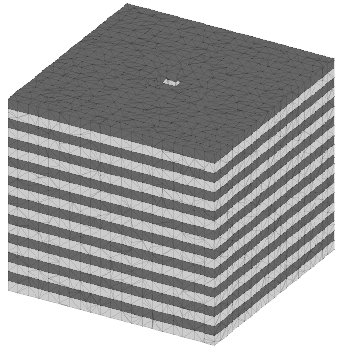
\includegraphics[width=5cm,height=5cm]{figures/Amir_Percolation_Setup_a.png}
\subcaption{}
\label{fig:Amir_Percolation_Setup_a}
\end{subfigure}
\hfill
\begin{subfigure}[c]{0.48\textwidth}
\centering
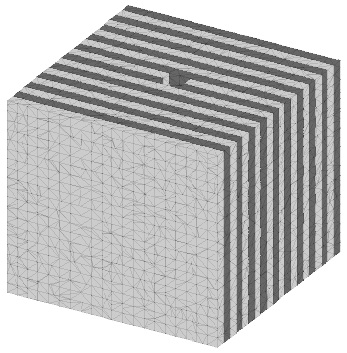
\includegraphics[width=5cm,height=5cm]{figures/Amir_Percolation_Setup_b.png}
\subcaption{}
\label{fig:Amir_Percolation_Setup_b}
\end{subfigure}
\caption{The generated 3D domain in lattice model for the (a) $1^{st}$ stress configuration, and (b) $2^{nd}$ stress configuration}
\end{figure}

\begin{figure}[!ht]
\begin{subfigure}[c]{0.48\textwidth}
\centering
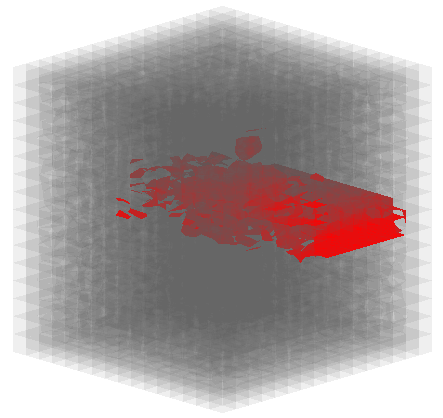
\includegraphics[width=5cm,height=5cm]{figures/Amir_ME2_B_Fracture_a.png}
\subcaption{}
\label{fig:Amir_ME2_B_Fracture_a}
\end{subfigure}
\hfill
\begin{subfigure}[c]{0.48\textwidth}
\centering
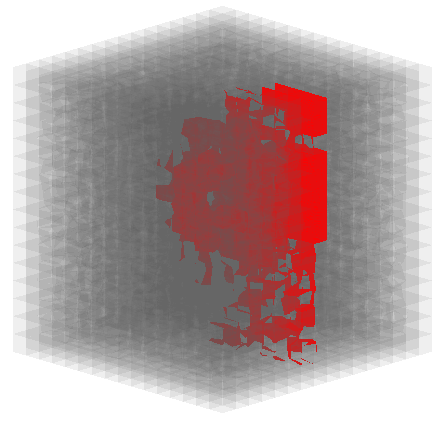
\includegraphics[width=5cm,height=5cm]{figures/Amir_ME2_B_Fracture_b.png}
\subcaption{}
\label{fig:Amir_ME2_B_Fracture_b}
\end{subfigure}
\caption{The fracking surfaces (red) for the (a) $1^{st}$ , and (b) $2^{nd}$ stress configurations}
\end{figure}

\begin{figure}[!ht]
\label{fig:VPF_ME2_B_init}
\begin{subfigure}[c]{0.48\textwidth}
\centering
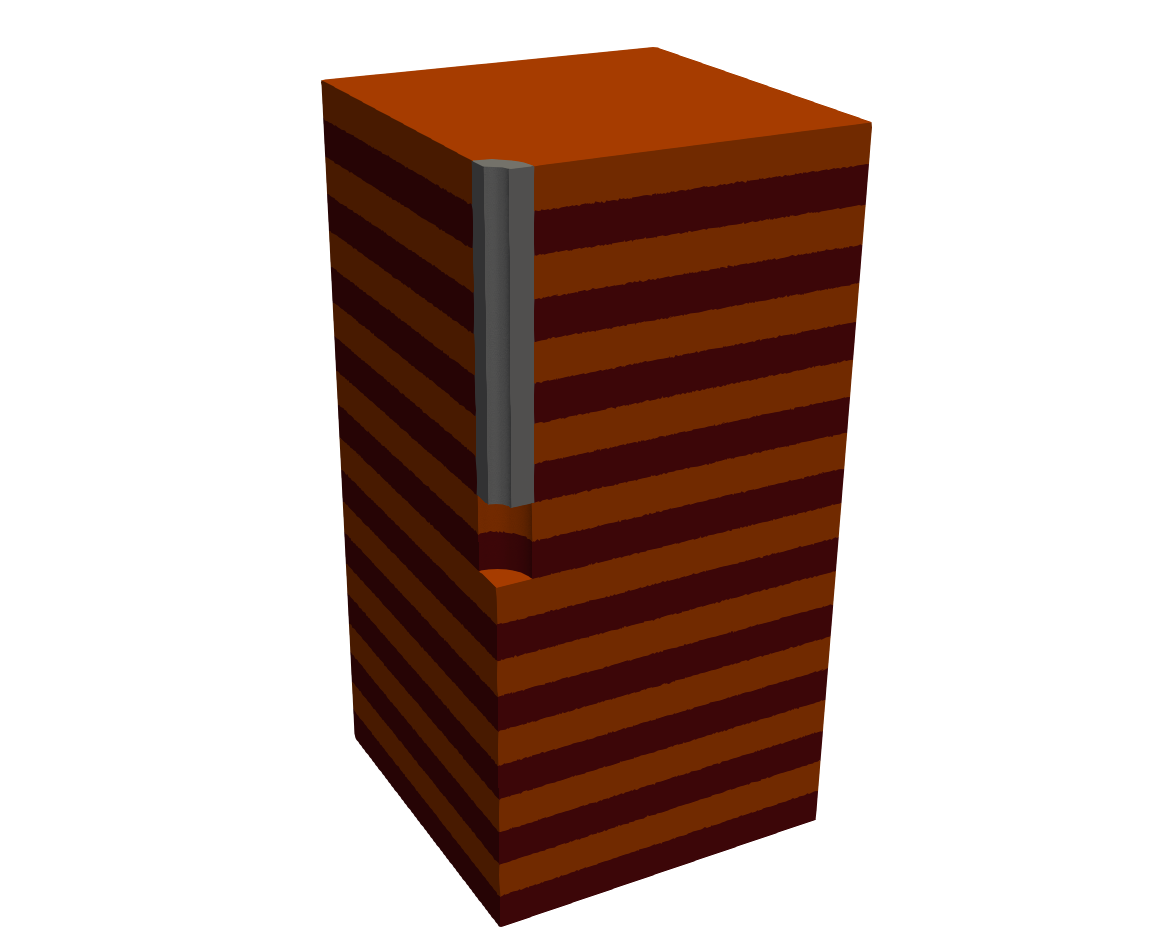
\includegraphics[width=5cm,height=5cm]{figures/ME2b_init_para.png}
\subcaption{}
\end{subfigure}
\hfill
\begin{subfigure}[c]{0.48\textwidth}
\centering
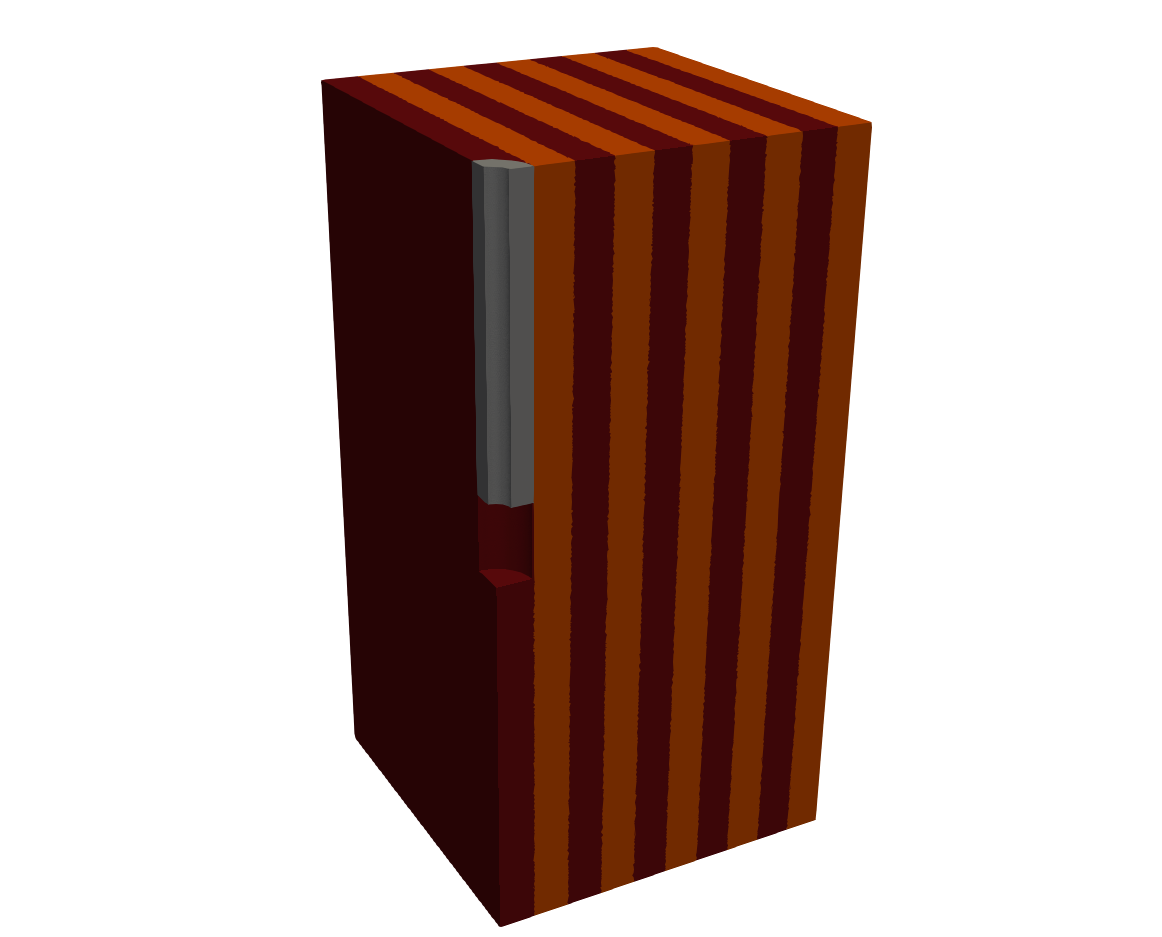
\includegraphics[width=5cm,height=5cm]{figures/ME2b_init_orth.png}
\subcaption{}
\end{subfigure}
\caption{3D computation domain of VPF for (a) $1^{st}$ stress configuration, and (b) $2^{nd}$ stress configuration.}
\end{figure}

\subsubsection*{Finite-Element-Model: Variational Phase-Field (VPF)}
Using the variational phase-field model presented in this study, impacts of the anisotropy induced by the lamination parallel and orhtogonal of the Opalinus claystone will be studied through 3D computational domains (Figs~\ref{fig:VPF_ME2_B_init}).



%------------------------------------------------------------------------------
\subsection{Results and discussion}
The experimental results form the fluid driven percolation tests on Opalinus claystone show the effect of the anisotropy on fracking paths and stress distribution. The fracking and leakage through the weak bond along the embedded layers is observed. However, more experimental data under different principle stress configurations are required to detect and analyse the stress distribution and the frack paths dependency on the anisotropy. For both samples tested here the fracking stress was higher than the applied minimum principle stress. For a $1^{st}$ stress configuration, the fracking pressure was much higher than applied maximum principle stress, which can be due to an error in the experimental results. The lack of the pre-defined notch during the sample preparation also can lead to higher fracking stresses. The fracking in $2^{nd}$ stress configuration was subtle and no pressure drop is recorded. The increase in the flow volume at the borehole pressure of 10 $MPa$ indicate the initiation of the fracking process. The dual lattice model is implemented to simulate the hydraulic fracking in Opalinus claystone. The anisotropy is implemented in the model, where the bond strength between the embedded layers is assumed to be 5 times weaker than a same layer bond. Due to this assumption which is found from Brazilian disk results (Sec.\ref{sec:Brazilian_Disk_Exp}), the fracking along the embedded layers is observed. The fracking pressures found to be higher than minimum principle stresses. However, more research for quantitative comparison of the results is needed. 


%------------------------------------------------------------------------------
